%%%%%%%%%%%%%%%%%%%%%%%%%%%%%%%%%%%%%%%%%
% Short Sectioned Assignment
% LaTeX Template
% Version 1.0 (5/5/12)
%
% This template has been downloaded from:
% http://www.LaTeXTemplates.com
%
% Original author:
% Frits Wenneker (http://www.howtotex.com)
%
% License:
% CC BY-NC-SA 3.0 (http://creativecommons.org/licenses/by-nc-sa/3.0/)
%
%%%%%%%%%%%%%%%%%%%%%%%%%%%%%%%%%%%%%%%%%

%----------------------------------------------------------------------------------------
%	PACKAGES AND OTHER DOCUMENT CONFIGURATIONS
%----------------------------------------------------------------------------------------

\documentclass[paper=a4, fontsize=11pt]{scrartcl} % A4 paper and 11pt font size

\usepackage[T1]{fontenc} % Use 8-bit encoding that has 256 glyphs
\usepackage[ngerman]{babel}
\usepackage{fourier} % Use the Adobe Utopia font for the document - comment this line to return to the LaTeX default
\usepackage{amsmath,amsfonts,amsthm} % Math packages
\usepackage{graphicx}
\usepackage[utf8]{inputenc}
\usepackage{listings}
\usepackage[section]{placeins}
\usepackage{lipsum} % Used for inserting dummy 'Lorem ipsum' text into the template
\usepackage{float}
\usepackage{multicol}
\usepackage{titlesec}
\setcounter{secnumdepth}{4}
\setcounter{tocdepth}{4}

\titleformat{\paragraph}
{\normalfont\normalsize\bfseries}{\theparagraph}{1em}{}
\titlespacing*{\paragraph}
{0pt}{3.25ex plus 1ex minus .2ex}{1.5ex plus .2ex}

\usepackage{sectsty} % Allows customizing section commands
\allsectionsfont{\centering \normalfont\scshape} % Make all sections centered, the default font and small caps

\usepackage{fancyhdr} % Custom headers and footers
\pagestyle{fancyplain} % Makes all pages in the document conform to the custom headers and footers
\fancyhead{} % No page header - if you want one, create it in the same way as the footers below
\fancyfoot[L]{} % Empty left footer
\fancyfoot[C]{} % Empty center footer
\fancyfoot[R]{\thepage} % Page numbering for right footer
\renewcommand{\headrulewidth}{0pt} % Remove header underlines
\renewcommand{\footrulewidth}{0pt} % Remove footer underlines
\setlength{\headheight}{13.6pt} % Customize the height of the header

\numberwithin{equation}{section} % Number equations within sections (i.e. 1.1, 1.2, 2.1, 2.2 instead of 1, 2, 3, 4)
\numberwithin{figure}{section} % Number figures within sections (i.e. 1.1, 1.2, 2.1, 2.2 instead of 1, 2, 3, 4)
\numberwithin{table}{section} % Number tables within sections (i.e. 1.1, 1.2, 2.1, 2.2 instead of 1, 2, 3, 4)

\setlength\parindent{0pt} % Removes all indentation from paragraphs - comment this line for an assignment with lots of text

%----------------------------------------------------------------------------------------
%	TITLE SECTION
%----------------------------------------------------------------------------------------

\newcommand{\horrule}[1]{\rule{\linewidth}{#1}} % Create horizontal rule command with 1 argument of height

\title{	
\normalfont \normalsize 
\textsc{Karlsruhe Institute of Technology} \\ [25pt] % Your university, school and/or department name(s)
\horrule{0.5pt} \\[0.4cm] % Thin top horizontal rule
\huge Maschinelles Lernen II\\ % The assignment title
\horrule{2pt} \\[0.5cm] % Thick bottom horizontal rule
}

\author{Manuel Lang} % Your name

\date{\normalsize\today} % Today's date or a custom date

\DeclareMathOperator*{\argmax}{arg\,max}
\DeclareMathOperator*{\argmin}{arg\,min}

\begin{document}

\maketitle % Print the title
\newpage

{\small\tableofcontents}
\newpage

%----------------------------------------------------------------------------------------
%	PROBLEM 1
%----------------------------------------------------------------------------------------

\section{Einführung}

\subsection{Einordnungskriterien für die Einordnung von Grundverfahren}

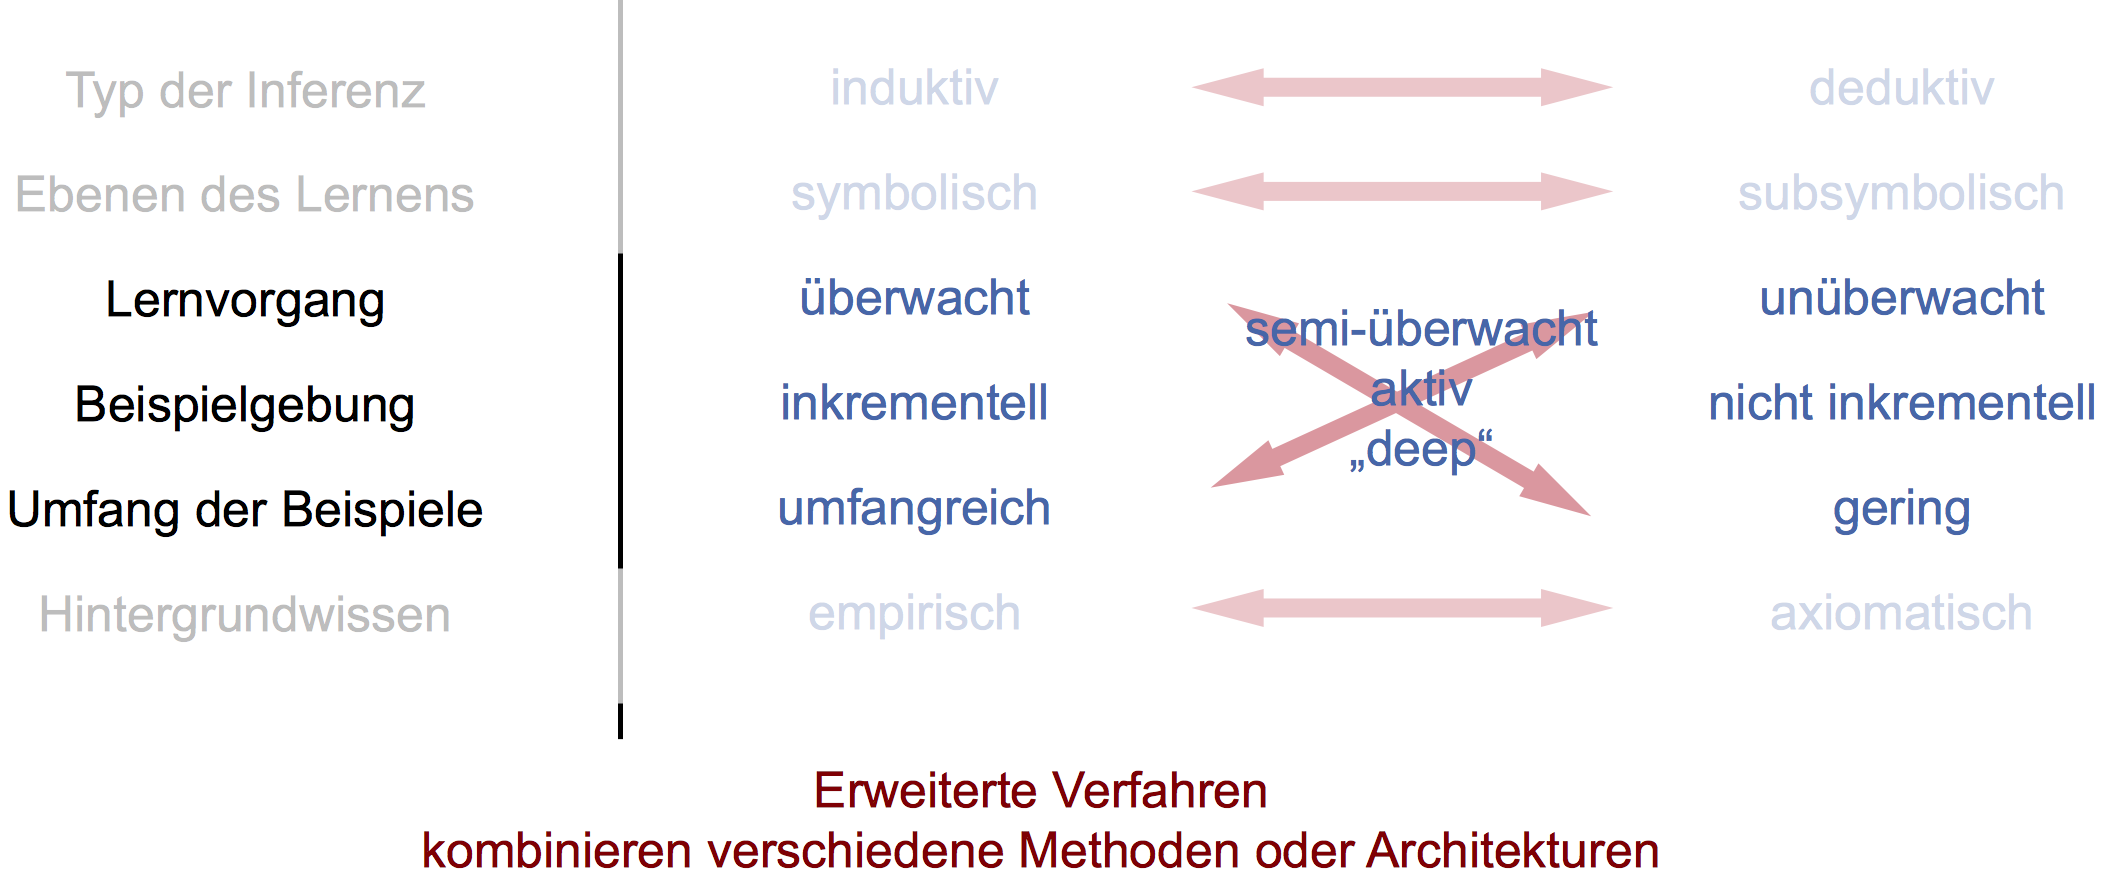
\includegraphics[width=\textwidth]{imgs/criteria}

\subsection{Komponenten eines lernenden Systems}

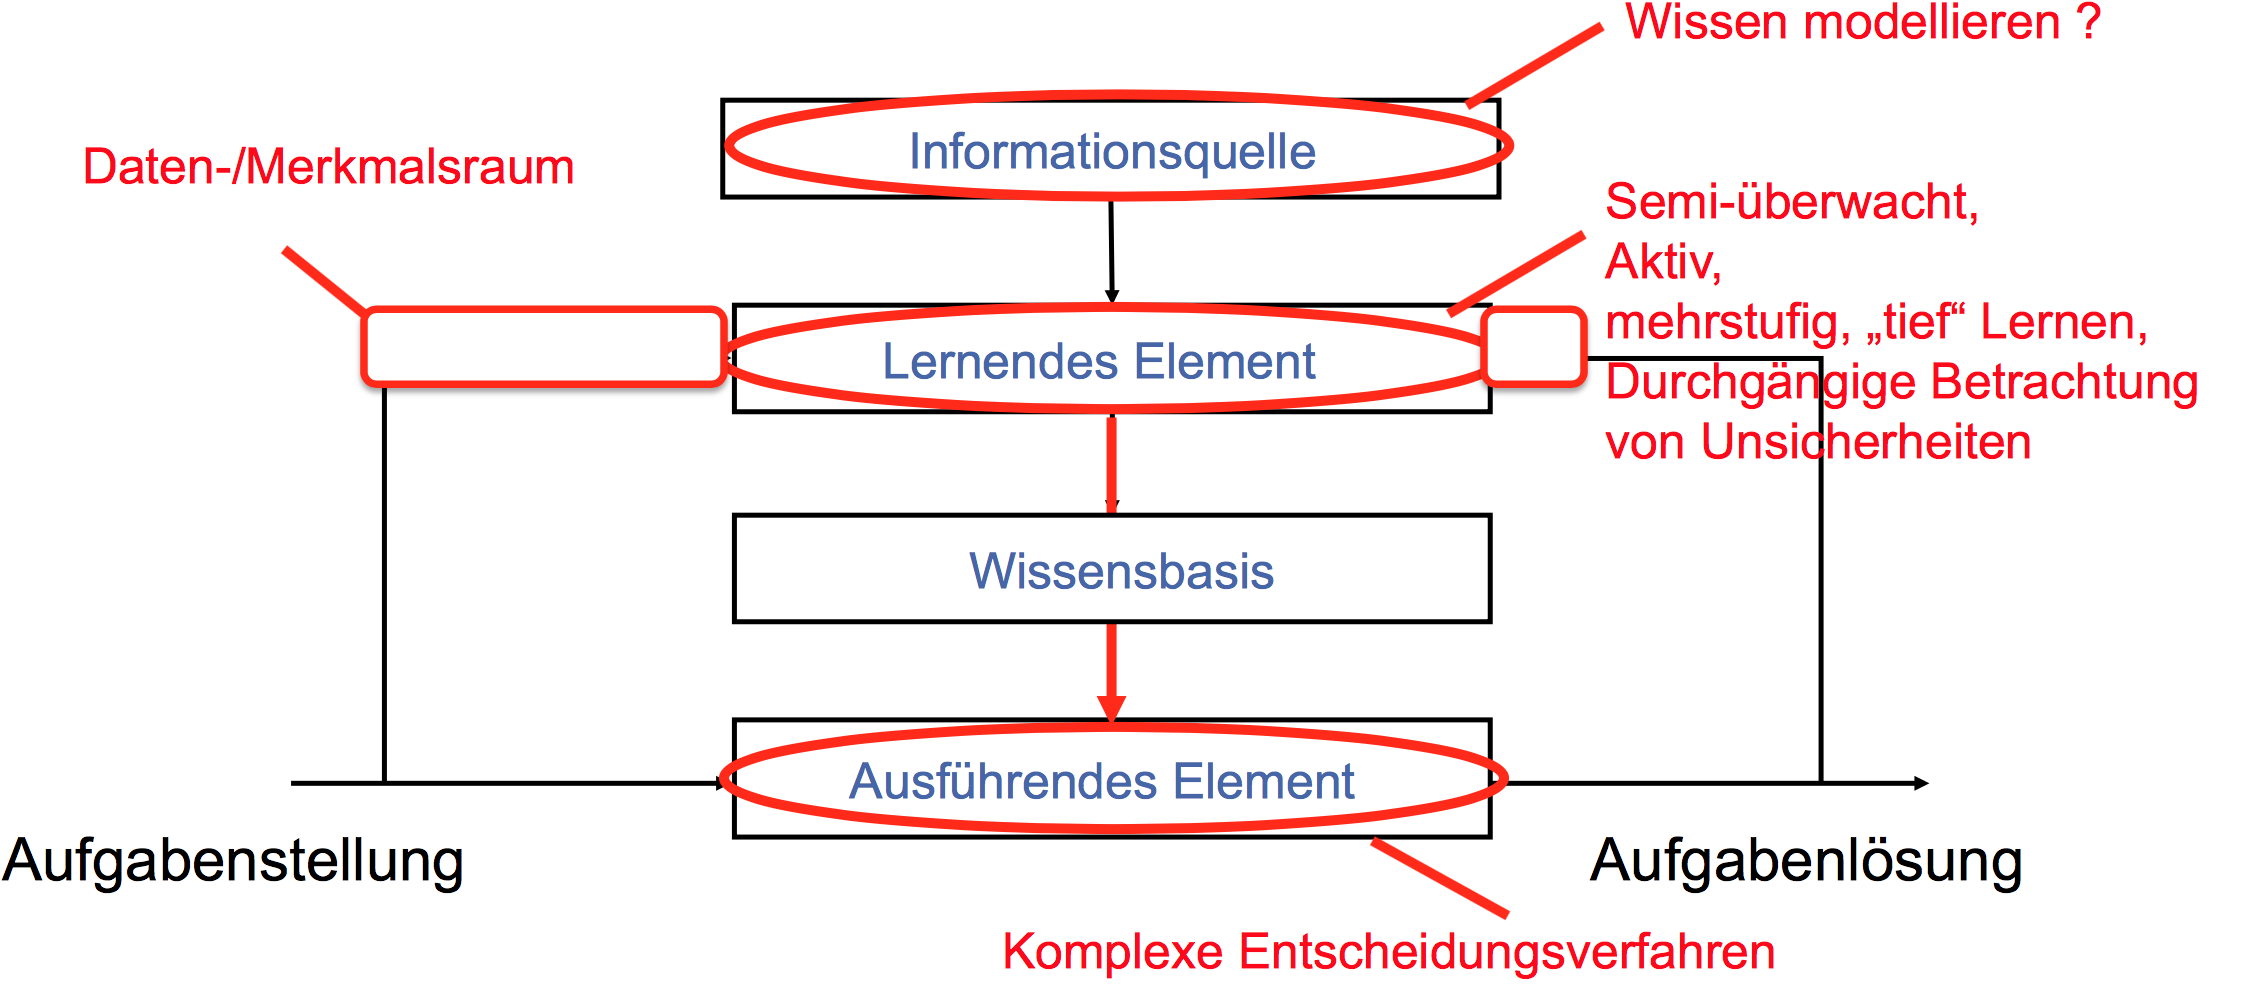
\includegraphics[width=\textwidth]{imgs/components}
\newpage
\section{Semiüberwachtes Lernen}

\subsection{Definitionen}

\subsubsection{Das SSL-Problem}

\begin{itemize}
\item Überwachtes Lernen
\begin{itemize}
\item Gelabelte Trainingsdaten: Paare $(X,Y)$
\item Finde Funktion $X$ (Merkmalsraum) $\implies Y$ (z.B. Klassen)
\end{itemize}
\item Unüberwachtes Lernen
\begin{itemize}
\item Ungelabelte Daten aus Merkmalsraum $X$
\item Strukturen und Labels der Daten finden (Ballungsanalyse), oft auch Dichte-(Träger)-Schätzung
\end{itemize}
\item Semi-Überwachtes Lernen
\begin{itemize}
\item wenige gelabelte Lerndaten, viele ungelabelte Daten
\item Finde Funktion $X$ (Merkmalsraum) $\implies Y$ (z.B. Klassen)
\item Bessere Performanz mit minimalen Kosten wird angestrebt: ungelabelte Daten sind billig (Sprache, Videoaufzeichnung, Bilder/Videos im Web), gelabelte Daten sind relativ teuer und schwer zu erzeugen (Annotation von Sprache 400h für 1h Sprachdaten, Experten nötig, Annotationen fehleranfällig)
\end{itemize}
\item SSL: Verwendung von gelabelten und ungelabelten Daten um bessere Hypothese zu erzeugen
\item Bessere Hypothese heißt:
\begin{itemize}
\item SSL kann und sollte verglichen werden und besser sein als Ergebnis des überwachten Lernens mit ausschließlich gelabelten Daten und Ergebnis des unüberwachten Lernens mit allen Lerndaten (ohne Labels).
\item Vergleich mit diesen beiden unteren Schranken liefert Informationen darüber, ob die Annahme, die beim semi-überwachten Lernen gemacht wird gilt oder ob der verwendete Ansatz (Modell) diese verletzt.
\end{itemize}
\end{itemize}
\newpage
\subsubsection{Grundannahmen}

\begin{itemize}
\item Gleichmäßigkeit für überwachtes Lernen (Smoothness Assumption): Wenn zwei Datenpunkte $x_1, x_2$ nahe beieinander sind, dann sollten auch die Ausgaben $y_1, y_2$ ähnlich sein.
\item Gleichmäßigkeit für Semi-überwachtes Lernen: Wenn zwei Datenpunkte $x_1, x_2$ in einer dichten Region nahe beieinander sind, dann sollten auch die Ausgaben $y_1, y_2$ ähnlich sein $\implies$ wenn zwei Datenpunkte durch einen Pfad hoher Dichte verbinden sind (i.A. gehören dem gleichen Cluster an), dann sind ihre Ausgaben ähnlich\\
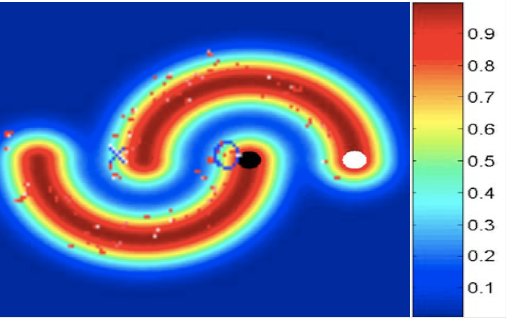
\includegraphics[width=0.6\textwidth]{imgs/density}
\item Cluster oder Dichte-Annahme: Wenn zwei Datenpunkte im selben (dichten) Cluster sind, dann sind sie in derselben Klasse $\implies$ eine Trennung sollte in einer Region niedriger Dichte (zwischen den Clustern liegen)
\item Manigfaltigkeit-Annahme (Manifold Assumption): Hochdimensionale Daten haben eine Abbildung in einen i.A. anders dimensionalen Raum (Manigfaltigkeitsraum) in dem sich ihre Strukturen abbilden (unterscheiden/erhalten) $\implies$ Dieser Raum kann dann für die Berechnung des geodäsischen Abstands benutzt werden, approximative Implementierung der Gleichmäßigkeitsannahme
\end{itemize}

\subsubsection{Formalisierung}

\begin{itemize}
\item Instanzen: Feature-Vektor $x \in X$, Label $y \in Y$
\item Hypothese: $h: X \implies Y$
\item Gelabelte Daten: $(X_l, Y_l) = {(x_{1:l}, y_{1:l})}$
\item Ungelabelte Daten: $X_u = {x_{l+1:n}}$
\item Üblicherweise gilt $l << n$
\item Neue Daten $X_{test} = {x_{n+1:...}}$
\end{itemize}

\subsubsection{Induktiv vs Transduktiv}

\begin{itemize}
\item Gegeben die Daten
\begin{itemize}
\item Gelabelte und ungelabelte Lerndaten
\item Ungelabelte Daten
\end{itemize}
\item Induktives Lernen (d.h. auch semi-überwachtes Lernen): Ziel ist das Schätzen einer Hypothese $h: X \implies Y$, die auch unbekannte Daten gut abbildet
\item Transduktives Lernen: Ziel ist das Labeln der ungelabelten Daten (kann auch das Labeln neuer Daten sein), das Finden einer Hypothese ist nicht das Ziel, kann aber erfolgen
\end{itemize}

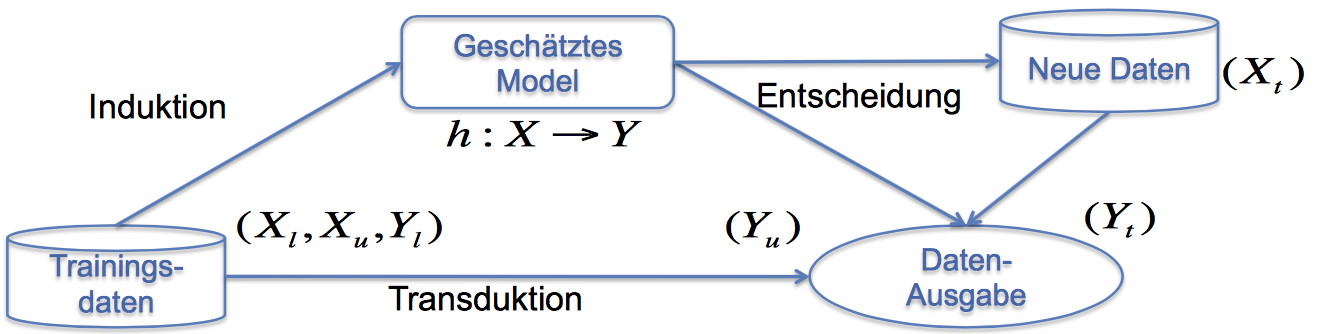
\includegraphics[width=\textwidth]{imgs/indvstran}

\subsubsection{Problemstellungen}

\begin{itemize}
\item Überwachtes Lernen (Klassifikation/Regression): ${(x_1{1:n}, y_{1:n})}$
\item Semi-überwachte Klassifikation/Regression: ${(x_{1:l}, y_{1:l}), x_{l+1:n}, x_{test}}$
\item Transduktive Klassikation/Regression: ${(x_{1:l}, y_{1:l}, x_{l+1:n})}$
\item Semi-überwachtes Clustern: ${x_{1:n}, must-links, cannot-links}$
\item Unüberwachtes Lernen: ${x_{1:n}}$
\item \textbf{Fokus in ML II: Algorithmen für die Klassifikation}
\end{itemize}
\newpage
\subsection{SSL-Methoden}

\subsubsection{Self-Learning und Co-Training}

\paragraph{Selbst-Lernen / Self-Training}

\begin{itemize}
\item Grundidee: Sukzessive Verwenden der ungelabelten Daten, die durch die gelernte Hypothese eine hohe Konfidenz der Prädiktion erreichen (Konfidenz $\approx$ Wahrscheinlichkeit der Klassenzugehörigkeit)
\item Grundalgorithmus (Wrapper): Wiederhole
\begin{itemize}
\item Trainieren mit gelabelten Daten: $h \Leftarrow (X_l, Y_l)$
\item Auswerten der ungelabelten Daten $h(x), \forall x \in X_u$
\item Einfügen konfidenter Daten zu den Trainingsdaten\\ $(X_l, Y_l) \Leftarrow (X_l, Y_l) \cup {(x, h(x)) | x \in X_u, h(x) - hohe Konf.}$
\end{itemize}
\item Variationen - Hinzunehmen neuer Daten: nur konfidente neue Beispiele, alle Beispiele, mit Gewichtung anhand der Konfidenz (Lernverfahren muss dies erlauben)
\item weit verbeiret und vermutlich älterester SSL-Ansatz (1965-1970)
\begin{itemize}
\item Wrapper Algorithmus anwendbar für alle überwachten Lernmethoden
\item Startet auf gelabelten Daten
\item In jeder Iteration werden ungelabelte Daten gelabelt, abh. von der Entscheidungsfunktion
\item Bezeichnung: self-learning, self-labeling, decision-directed learning
\end{itemize}
\item Diskussion
\begin{itemize}
\item Kann effektiv sein
\item Aber es ist nicht genau bestimmt, wie das Ergebnis ist (und abhängig von der Methode des überwachten Lernens)
\item Nicht methodisch festgelegt, welche Annahmen über das Problem getroffen werden
\end{itemize}
\item Vorteile
\begin{itemize}
\item Sehr einfache semi-überwachte Lernmethode
\item Wrapper - passend zu existenten auch komplexten Klassifikatoren
\item Oft angewandt in realen Anwendungen wie z.B. Sprachanalayse
\end{itemize}
\item Nachteile
\begin{itemize}
\item Frühe Fehlentscheidungen können sich verstärken - Heuristische Lösung: Daten un-labeln sofern ihre Konfidenz unter einen Schwellwert fällt
\item Generelle Analyse kompliziert - nur für Spezialfälle ist eine geschlossene und formlose Analyse möglich, in Spezialfällen entspricht Selbst-Lernen dem EM-Ansatz
\end{itemize}
\end{itemize}

\paragraph{Mit-Lernen / Co-Training}

\begin{itemize}
\item Annahme: Features können in 2 voneinander unabhängige Mengen aufgeteilt werden $x = [x^{(1)}, x^{(2)}]$ (Feature-Split), somit gilt für jeden Vektor: Jede Untermenge ist ausreichend um eine gute Lernmaschine (im weiteren Klassifikator) einzutrainieren
\item Lernansatz: Verwenden den Wrapper-Ansatz mit 2 unabhängigen Klassifikatoren für beide Featuremengen $(X_l^{(1)}, Y_l) \implies h^{(1)}, (X_l^{(2)}, Y_l) \implies h^{(2)}$ (z.B. Bild und Textklassifikation von Webseiten)
\item Vorteile
\begin{itemize}
\item Wrapper Methode - anwendbar auf alle existierenden Klassifikatoren
\item Weniger anfällig für Missentscheidungen als Selbstlernen
\end{itemize}
\item Nachteile
\begin{itemize}
\item Natürliche Featureaufteilung ggf. nicht vorhanden
\item Modelle die die vollständige Featuremenge benutzen erreichen oft bessere Ergebnisse
\end{itemize}
\item Varianten
\begin{itemize}
\item Fake Feature Split: zufällig, künstliche Aufteilung der Merkmale, Co-Training wie bisher
\item Multi-View-Ansatz: kein Feature Split, trainiere mehrere Klassifikatoren, Klassifizierung der ungelabelten Daten mit allen Klassifikatoren, verwende Mehrheitsentscheidung für neue Labels
\item Co-EM: Nutzung aller Daten, jeder Klassifikator labelt die Daten $X_u$ probabilistisch, Daten $(x,y)$ werden probabilistisch genutzt mit Gewicht $p(y|x)$
\end{itemize}
\end{itemize}

\subsubsection{Generative probabilistische Modelle}

\begin{itemize}
\item Generative Algorithmen nutzen eine Schätzung der Verteilung der Daten für die Klassen $\Rightarrow$ zusätzliche Information der Verteilung der Daten ist sinnvoll.
\item Grundverfahren
\begin{enumerate}
\item Wähle ein generatives Modell $p(x,y|\theta)$
\item Finde Maximum Likelihood Schätzung (MLE) auf gelabelten und ungelabelten Daten $\theta^* = \argmax\limits_{\theta} p(X_l, Y_l, X_u | \theta)$ mit Expectation Maximization Algorithmus
\begin{itemize}
\item Starte mit MLE $\theta = {\pi_1, \pi_2, \mu_1, \mu_2, \Sigma_1, \Sigma_2}$ auf $(X_l,Y_l)$
\item E-Schritt
\begin{itemize}
\item Berechne Wahrscheinlichkeit für alle $x \in X_u, p(y|x,\theta) = \frac{\pi_y p(x|\theta_y)}{p(x|\theta)}$
\item Setze Label (je nach Maximum) $y_u = 1$ bzw. $y_u = 2$
\end{itemize}
\item M-Schritt
\begin{itemize}
\item Update von $\theta$ jetzt auch mit $(X_u,Y_u)$ (soft label)
\item A-priori-Klassenwahrscheinlichkeit = Anteil der Daten mit Klasse $i = \pi_i$
\item (gewichteter) Mittelwert der Klasse $i = \mu_i$
\item (gewichtete) Kovarianz der Daten der Klasse $i = \Sigma_i$
\end{itemize}
\item Iteriere
\item Kann als Sonderfall des Selbstlernens gesehen werden
\end{itemize}
\item Bestimme Klassenzugehörigkeit entsprechend der Bayes'schen Regel\\ $p(y|x,\theta^*) = \frac{p(x,y|\theta_y^*)}{\sum\limits_{y'}p(x,y'|\theta^*)} = \frac{p(x|\theta^*) p(y|X,Y)}{p(x|\theta^*)}$
\end{enumerate}
\item Grundsatz
\begin{itemize}
\item Maximierung von $p(X_l,Y_l,X_u|\theta)$
\item Verwende optimales Modell für die Trennung
\item EM ist nur eine Variante, andere Methoden existieren
\end{itemize}
\item Vorteile
\begin{itemize}
\item Klares, wohl definiertes Framework
\item Kann sehr effektiv sein wenn das Modell korrekt ist
\end{itemize}
\item Nachteile
\begin{itemize}
\item Verifikation der Korrektheit des Modells meist nicht möglich
\item EM kann zu lokalen Minima führen
\item Ungelabelte Daten können schaden wenn das Modell nicht korrekt ist
\end{itemize}
\end{itemize}

\subsubsection{Low-Density Separation / Dichte Trennung - ``Transduktive'' SVM}

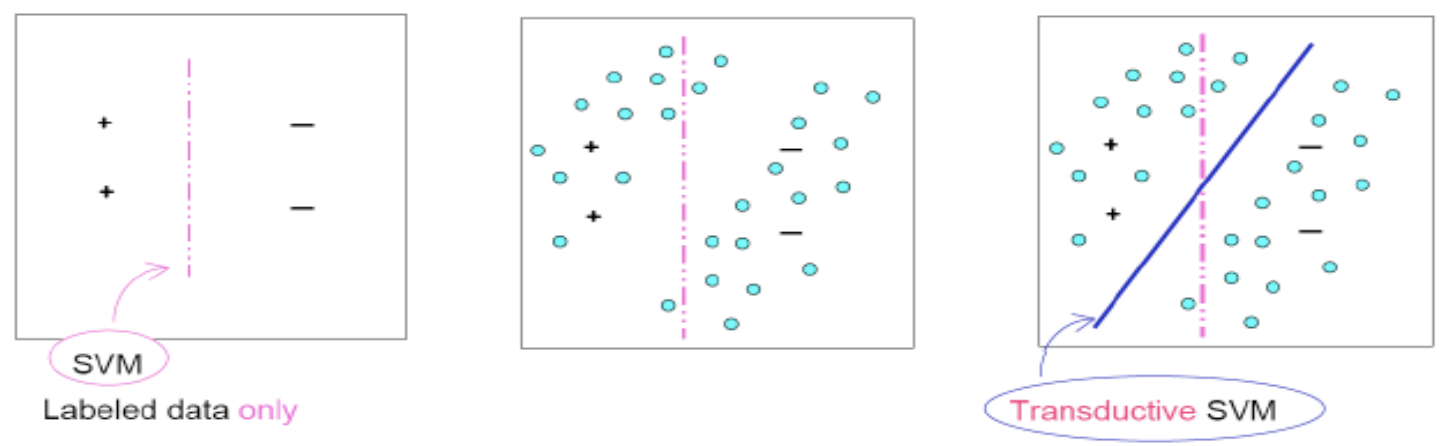
\includegraphics[width=\textwidth]{imgs/transsvm}

\begin{itemize}
\item Annahme: Ungelabelte Daten unterschiedlicher Klassen werden mit großen Rand getrennt - aber wie?
\item Naiver Ansatz: Alle $2^u$ Möglichkeiten der Labels v. $X_u = {x_{l+1:l+u}}$ betrachten, trainiere SVM für alle Möglichkeiten, wähle SVM mit größtem Rand
\item Besser: integriere ungelabelte Daten in das Optimierungsproblem
\item Realer Fehler: $R(w) = \int L(y, f(x; w)) p(x,y) dxdy$ mit der realen Verteilung der Daten $p(x,y)$
\item ``Transduktive'' SVM - Anpassung
\begin{itemize}
\item Einbinden der ungelabelten Daten
\begin{itemize}
\item Problem: $y_i$ unbekannt für alle ungelabelten Daten
\item Für korrekte Labels würde gelten: $y_i = sign f(x_i) for x_i \in X_u$
\item Hinge-Funktion für ungelabelte Daten: $(1-y_i f(x_i))_+ = (1 - |f(x_i|)_+$ weil $sign(f(x_i)) f(x_i) = |f(x_i)|$
\item Minimierungsproblem kann erweitert werden\\ $\min\limits_{w,b} {\frac{1}{2}||w||^2 + C_1 \sum\limits_{i=1}^{l}(1-y_i f(x_i)) + C_2 \sum\limits_{i=l+1}^n (1-|f(x_i)|)_+}$
\end{itemize}
\end{itemize}
\item SVM$^{light}$-Ansatz
\begin{itemize}
\item Heuristisches, iteratives Labeln mit Ausbalancierung
\item Trainiere SVM auf $(X_l, Y_l)$
\item Labeln von $X_u$ durch $f(x_i)$, Label $\hat{y_i} \Leftarrow -1/1$
\item Von $\tilde{C} \Leftarrow 10^-5 C_2$ bis $C_2$ (schrittweise iteratieren)
\begin{itemize}
\item Trainiere SVM mit\\ $\min\limits_{w,b} {\frac{1}{2}||w||^2 + C_1 \sum\limits_{i=1}^{l}(1-y_i f(x_i)) + C_2 \sum\limits_{i=l+1}^n (1-|f(x_i)|)_+}$
\item Tausche Labels $\hat{y_i}, \hat{y_j}$ wenn $\exists(i,j) switchable$
\end{itemize}
\item Bis keine tauschbaren Labels.
\end{itemize}
\item S$^3$VM (Semi-Supervised Support Vector Machines) probabilistische Sicht für überwachtes Lernen
\begin{itemize}
\item Wahrscheinlichkeit für die Ausgabe $y$ gegeben $x$: $p(y|x) = \frac{1}{(1+exp(-y f(x)))}$ mit $f(x) = w^T x + b$
\item Log-Gesamtwahrscheinlichkeit (über alle Daten): $\sum\limits_{i=1}^{l} log p(y_i|x_i,w,b)$
\item MAP-Training (inklusive Rand): $\max\limits_{w,b} \sum\limits_{i=1}^l log(\frac{1}{(1+exp(-y_i f(x_i)))}) - \lambda ||w||^2$ bzw. $\min\limits_{w,b} \sum\limits_{i=1}^l log(1+exp(-y_i f(x_i))) + \lambda_1 ||w||^2$
\item Wenn zwei Klassen gut trennbar sind, dann sollte $p(x|y)$ nahe 0 oder 1 sein für alle Instanzen ungelabelter Daten $\Rightarrow$ Entropie ist klein
\item Probabilistische Sicht führt zur Kostenfunktion
\item Entropie Betrachung / Regularisierung führt zur Kostenfunktion
\end{itemize}
\item ``Transduktive'' SVM/S$^3$VM - Diskussion
\begin{itemize}
\item Vorteile
\begin{itemize}
\item Anwendbar wenn SVM anwendbar
\item Klar formuliertes mathematisches Rahmenwerk
\end{itemize}
\item Nachteile
\begin{itemize}
\item Optimierungsproblem nicht mehr konvex
\item Optimierung - kompliziert
\item Lokale Minima
\item Schwächere Annahme (Dichte) als generative Modelle oder graphbasierte Methoden $\Rightarrow$ möglicherweise schlechtere Ergebnisse
\end{itemize}
\end{itemize}
\end{itemize}

\subsubsection{Graph basierte Modelle}

\textbf{Nicht in Vorlesung behandelt.}

\subsubsection{Änderung der Repräsentation}

\textbf{Nicht in Vorlesung behandelt.}

\section{Aktives Lernen}

\begin{itemize}
\item SSL
\begin{itemize}
\item Lernmaschine die mit wenigen überwachten und vielen unüberwachten Daten lernt
\item Annahme: zusätzliche Informationen über Datenverteilung ermöglicht Hypothesenfindung
\end{itemize}
\item Aktives Lernen (allgemeiner)
\begin{itemize}
\item Lernmaschine die ggf. mit wenigen überwachten aber wesentlich mit selektiv gewählten unüberwachten Daten lernt
\item Annahme: Einige Daten enthalten wesentlich mehr Informationen als andere
\end{itemize}
\end{itemize}

\subsection{Lernszenarien}

\begin{itemize}
\item Query Synthesis (Erzeugung synthetischer Daten) \\ 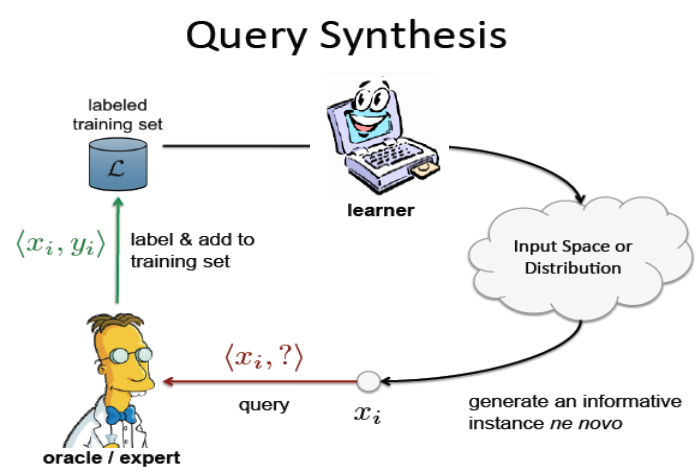
\includegraphics[width=0.6\textwidth]{imgs/qsyn}
\item Selective Sampling (Selektive Entnahme aus Daten-Strom) \\ 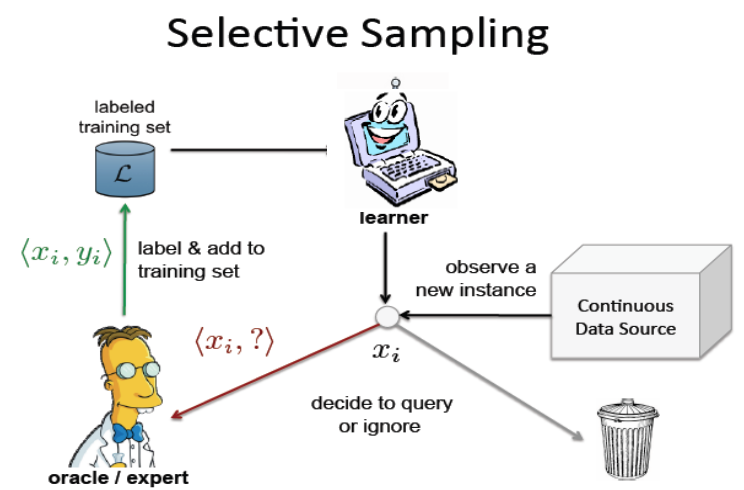
\includegraphics[width=0.6\textwidth]{imgs/ssam}
\item Pool Based (Auswahl aus Daten-Pool) \\ 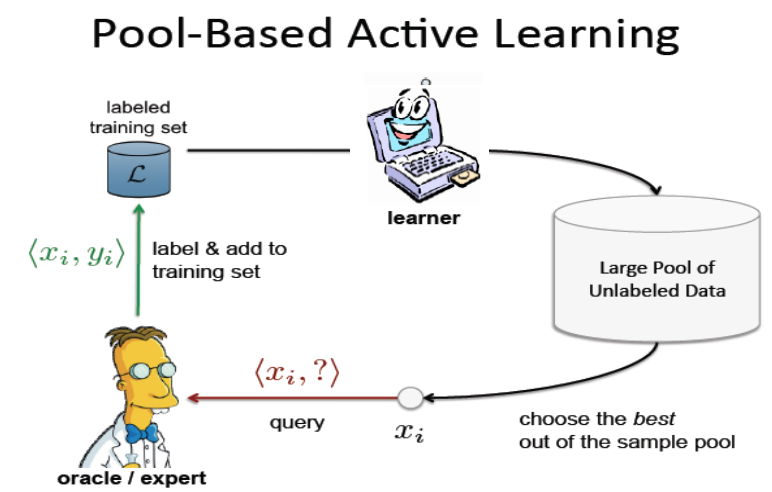
\includegraphics[width=0.6\textwidth]{imgs/pbas}
\end{itemize}

\subsection{Wahl der Lerndaten}

\begin{itemize}
\item Wähle die Daten für die Lernmaschine die größte Unsicherheit haben, z.B.
\begin{itemize}
\item Niedrigste Konfidenz (bester Klassenzugehörigkeit) bzw. höchste Unsicherheit $\phi_{LC}(x) = 1 - P_\theta(y^*|x)$
\item Kleinster Rand/Margin (bester Klassenzugehörigkeiten) $\phi_M(x) = P_\theta(y_1^*|x) - P_\theta(y_2^*|x)$
\item Entropie
\begin{itemize}
\item Als Erwartungswert des Informationsgehalts, definiert durch $E_y[-log P_\theta(y|x)]$
\item Maß (zu maximieren): $\phi_{ENT}(x) = - \sum\limits_y P_\theta(y|x) log_2 P_\theta(y|x)$
\end{itemize}
\item Für binäre Klassifikation sie diese Maße identisch, sonst nicht
\end{itemize}
\end{itemize}

\subsection{Version Space}

\begin{itemize}
\item Version Space: Menge aller Hypothesen die konsistent sind mit den Daten
\item Annahme: Um so größer der Version Space $v$ ist, um so schlechter ist jede mögliche Hypothese (Klassifikator)
\item Ziel beim aktiven Lernen: Reduktion des Version Space
\item Verfahren
\begin{itemize}
\item Simpler (naiver) Version Space Algorithmus
\begin{itemize}
\item Bestimme alle konsistenten Hypothesen oder bestimme $|v|$ analytisch
\item Optimales neues $x$ reduziert die Größe vo $v$ am stärksten
\begin{itemize}
\item als Erwartungswert über $y$ (weil Label zunächst unbekannt)
\item über alle Lerndaten inklusive der neuen Daten $L \cup <x,y>$ \\ $x^*_{VS} = \argmin\limits_x E_y |v^{L \cup <x,y>}|$
\end{itemize}
\item Idealerweise lässt sich der Version Space halbieren
\item Binäre Suche implementiert dies in 1D
\item Problem - effiziente Realisierung
\begin{itemize}
\item $V$ kann sehr groß werden oder ist analytisch nicht beschreibbar
\item Idee: Extremen des Hypothesenraums betrachten, wenn die Modelle sich stark widersprechen -> Daten (mit hoher Unsicherheit) reduzieren $v$
\item Allgemeiner Ansatz: Query-by-Committee
\end{itemize}
\end{itemize}
\item Query-by-Committee (QBC)
\begin{itemize}
\item Allgemeiner Ansatz
\begin{itemize}
\item Trainiere eine Menge $C$ von Maschinen (Klassifikatoren)
\item $C$ kann beliebiger Kardinalität sein
\item Wähle neue Daten wenn die Hypothesen (Klassifikatoren) widersprüchlich sind
\end{itemize}
\item Selektive Entnahme
\begin{itemize}
\item Beobachte neue Instanzen (Auswerten)
\item Abfrage falls Widerspruch
\item Neutrainieren, Iterieren
\end{itemize}
\item Pool-based Lernen
\begin{itemize}
\item Messung des Widerspruchs für alle Instanzen x
\item Ranking
\item Abfrage der k widersprüchlichsten Instanzen
\item Neutrainieren, Iterieren
\end{itemize}
\item Design
\begin{itemize}
\item Wahl des Ausschusses $C$ z.B. sampling von zulässigen Modellen geg. Lerndaten entsprechend $P(\theta|L)$ oder Lernen der Modelle <- Datenabhängig
\item Bestimmung des Widerspruchs einfach (z.B. XOR) oder korrekt - Betrachten der Einzelentscheidungen als Wahrscheinlichkeitsverteilung und Unsicherheitsmaß darauf anwenden, z.B. Entropie
\end{itemize}
\end{itemize}
\end{itemize}
\item Ausreißerproblem
\begin{itemize}
\item Problem: Eine Instanz kann widersprüchlich sein weil es sich um einen Ausreißer handelt, Ausreißer sind nicht geeignete Lerndaten
\item Mögliche Lösung: Gewichten der Unsicherheit einer Instanz x anhand der Dichte im Datenraum
\end{itemize}
\item Aktives Lernen mit SVM - Version Space
\begin{itemize}
\item Gegeben ungelabelte Instanzen (-> Hyperebenen in $H$) suchen wir diejenigen, die den VS maximal verringern
\item Einfache Lösung Simple Margin: Daten deren entsprechende Hyperbene die Hyperkugel gültiger Gewichtsvektoren möglichst zentral schneiden, dies sind die Daten die im nächsten zur Trennhyperebene im Merkmalsraum liegen
\item Besser: Nutzen der Eigenschaft, dass der SVM Rand proportional zur Version Space Fläche ist 
\item MaxMinMargin: Für jeden Datenpunkt berechne den Rand $m+$ und $m-$ nach potentieller Teilung in $V+$ und $V-$, Abfragen der Instanz $x = \argmax\limits_x min(m+,m-)$
\item Ratio Margin: Für jeden Datenpunkt berechne den Rand $m+$ und $m-$ nach potentieller Teilung in $V+$ und $V-$, Abfragen der Instanz $x = \argmax\limits_x min(\frac{m-}{m+},\frac{m+}{m-})$
\end{itemize}
\item Vorteile
\begin{itemize}
\item Anwendbar wenn SVM anwendbar
\item Klar formuliertes mathematisches Rahmenwerk
\item Berechnung des Randes jeweils nach Trainieren der SVM möglich
\item Praktische Ergebnisse zeigen, dass aktive SVM besser als passive SVM
\end{itemize}
\item Nachteile: MinMax und Ratio sind aufwändig in der Berechnung
\end{itemize}

\section{Tiefes Lernen}

\subsection{A temporary disgression}

\begin{itemize}
\item Vapnik und Kollegen entwickeln die ``very clever type of pereception'' [Hinton] - Support Vector Machine: ``a clever optimization technique is used'', ``but it's just a perceptron and has all the same limitations''
\item Hinton: ``In the 1990's, many researchers abandoned neural networks with multiple adaptive hidden layers because Support Vector Machines worked better.''
\item Problem von Backpropagation
\begin{itemize}
\item Überwachtes Lernen benötigt zu viele Trainingsdaten mit Zielwerten, aber die meisten realen Daten sind ohne Zielwerte
\item Performanz skaliert oft nicht wirklich gut: sehr langsames Lernen (Konvergenz) in Netzen mit vielen Hidden Layern <- diese werden leider benötigt
\item Lokale Minima
\item Overfitting
\end{itemize}
\item Positive Aspekte von Backpropagation
\begin{itemize}
\item Effizienz und Einfachheit (z.B. Gradienten-Abstieg für das Backprop Lernen) -> Ziel: beibehalten!
\item Aber: Die Struktur der (Input) Daten ist wichtig und sollte gelernt werden, Ziel: Generatives Modell nutzen!
\end{itemize}
\end{itemize}

\subsection{Definition tiefe Netze/Lernverfahren}

\begin{itemize}
\item Hinton: ``It is deep, if it contains at least two layers with non-linear transformations.''
\item LeCun (additional): ``It is deep, if it represents a feature hierarchy.''
\end{itemize}

\subsection{Einteilung Lernverfahren}

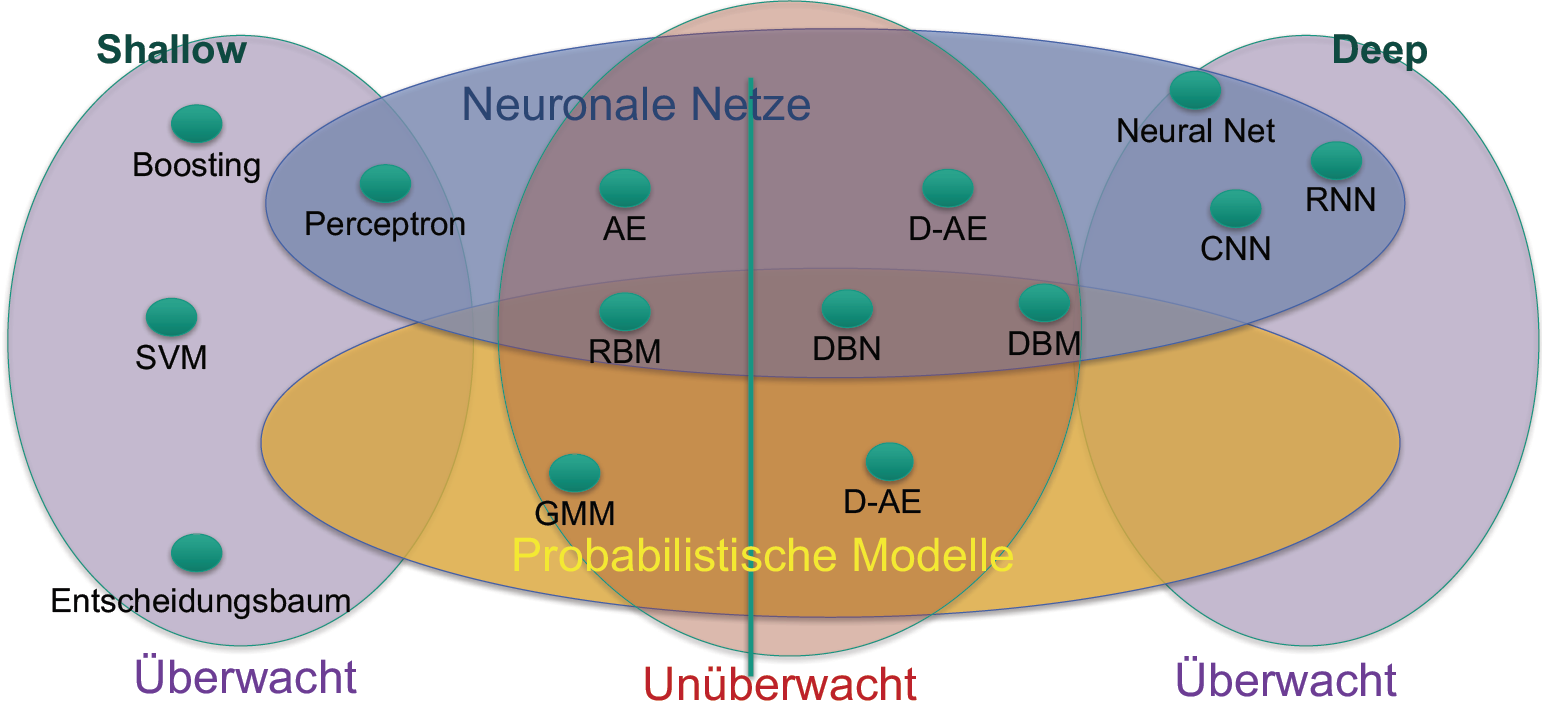
\includegraphics[width=\textwidth]{imgs/einteilung}

\subsection{Belief Netze}

\begin{itemize}
\item Ein Belief Netz ist ein gerichteter azyklischer Graph mit stochastischen Variablen (graphisches probabilistisches Modell).
\item Einige Variable sind beobachtbar (Evidenzen, Daten)
\item Inferenz-Problem: Schließen auf den Zustand der verdeckten Variablen
\item Lern-Problem: Anpassen der Variablen um das Netz zu befähigen beobachtete Daten generieren zu können
\item Einfaches Netz mit stochastischen binären Einheiten (Bernoulli Variablen)
\begin{itemize}
\item Mögliche Zustände der Knoten: 1 oder 0
\item Aktivierungswahrscheinlichkeit: bestimmt durch den gewichteten Input von anderen (Vorgänger) Einheiten (plus Bias) $b_i + \sum\limits_j s_j w_{ji}$, z.B. für sigmoide Einheiten entsprechend der Sigmoid Regel: $p(s_i = 1) = \frac{1}{1+exp(-b_i - \sum\limits_j s_j w_{ji})}$
\end{itemize}
\item Lernen in ``Deep'' Belief Nets
\begin{itemize}
\item Einfach (unbiased) Beispiele an den Endknoten zu generieren um zu sehen woran das Netz ``glaubt'' -> Belief Net
\item Schwer die a-posteriori Wahrscheinlichkeit für alle Konfigurationen der verdeckten Ursachen zu inferieren
\item Wie kann man dann in Deep Belief Netzen mit vielen Ebenen und Millionen von Parametern lernen?
\end{itemize}
\item Lernen für Sigmoide Belief Netze
\begin{itemize}
\item Lernen einfach wenn Daten der verdeckten Zustände (samples der a-posteriori Verteilung) gegeben der beobachteten Daten vorliegen
\item Idee des Lernens: Für jede Einheit: Maximiere die Wahrscheinlichkeit, dass der beobachtete Zustand $s_i$ von den binären Zuständen der Vorgänger generiert wird (Log Likelihood)
\item Problem: Wenn überhaupt nur für unterste Ebenen (micht sichtbaren Daten) möglich
\end{itemize}
\end{itemize}

\subsection{Restricted Boltzmann Maschinen (RBM)}

\begin{itemize}
\item Verbindung der binären stochastischen Einheiten in einem gerichteten azyklischen Graphen führt zu einem Sigmoid Belief Netz -> problematisch
\item Verbindung der binären stochastischen Einheiten mit symmetrischen Verbindungen führt zu einer Boltzmann Maschine -> bei Restriktion der Verbindung kann eine Boltzmann Maschine (gut) gelernt werden
\item Beschränkung der Verbindungen der Restricted Boltzmann Machine  um lernen zu können: nur ein hidden Layer, keine Verbindung zwischen Einheiten gleicher Layer
\item In einer RBM sind die hidden Einheiten unabhängig, wenn die beobachtbaren Variablen (Zustände) gegeben sind: Man erhält ``einfach'' den Zustand (sample der a-posteriori Verteilung) der hidden Einheiten gegeben ein Daten-Vektor <- sigmoid-Regel (aufwärts), wesentlicher Vorteil gegenüber den gerichteten Belief Netzen
\end{itemize}

Lernalgorithmen für RBM
\begin{itemize}
\item Maximum Likelihood Lernalgorithmus
\begin{itemize}
\item Start mit einem Trainingsvektor an den sichtbaren Einheiten
\item Alternieren zwischen update aller sichtbaren Einheiten (parallel). (Implementiert alternating Gibbs <- MCMC Ansatz um ein sample der Daten zu erhalten)
\item Dann gilt (Gradient): $\Delta w_{ij} \approx \frac{\partial log p(v)}{\partial w_{ij}} = <v_i h_j>^0 - <v_i h_j>^\infty$
\end{itemize}
\item Schneller Lernalgorithmus für RBM - Contrastive divergence learning
\begin{itemize}
\item Start Trainingsvektor an den sichtbaren Einheiten
\item Update aller hidden Einheiten - parallel
\item Update aller sichtbaren Einheiten (parallel) um eine Rekonstruktion zu erhalten
\item Update der hidden Einheiten
\item Update der Gewichte (nach update der hidden Einheiten): $\Delta w_{ij} = \epsilon (<v_i h_j)^0 - <v_i h_j>^1)$
\item Entspricht nicht ganz dem Gradienten des log likelihood aber funktioniert gut
\end{itemize}
\end{itemize}

\subsection{Tiefe Netze mit RBM (DBM)}

\begin{itemize}
\item Grundidee: mehrere RBM stapeln
\item Trainieren des layer, welche die Eingaben direkt von den Pixeln enthält ($W_1$)
\item Dann Aktivierung der trainierten Merkmale so verwenden als wären es Pixel und Lernen der zweiten verdeckten Schicht ($W_2$) usw.
\item Es kann gezeigt werden, dass jedes Mal wenn eine weitere Schicht hinzukommt, die untere Schwelle des log-likelihood der trainierten Daten erhöht wird (Beweis ist nicht trivial).
\item Äquivalenz zwischen RBM und gerichteten Deep Netzen
\end{itemize}

\subsubsection{Wieso funktioniert greedy Lernen?}

\begin{itemize}
\item Die Gewichte W, in der unteren Ebene des RBM definieren $p(v|h)$
\item Es gilt für die (untere) RBM: $p(v) = \sum\limits_h p(h) p(v|h)$
\item Verbesserung von $p(h)$ wird $p(v)$ verbessern
\item Um $p(h)$ zu verbessern benötigen wir ein besseres Modell um die a-posteriori Wahrscheinlichkeit der hidden Einheiten zu generieren <- d.h. die oberen RBM lernen
\end{itemize}

\subsubsection{Fine-tuning des Lernens: contrastive ``wake-sleep'' Algorithmus}

\begin{itemize}
\item Nach Lernen der einzelnen Layer -> Verbesserung durch fine-tuning
\item Lösen der symmetrischen Bindung zwischen den auf- und abwärts-Gewichten
\item Algorithmus
\begin{enumerate}
\item Wake (Aufwärtsschritt): Starte Anregung mit sichtbaren Daten, Anpassen der top-down Gewichte um die Aktivität der Merkmale in tiefere Ebenen zu rekonstruieren.
\item Einige Iterationen in der höchsten RBM -> Anpassen der Gewichte in der obersten RBM
\item Sleep (Abwärtsschritt): Anpassen der bottom-up Gewichte um die Aktivität der Merkmale in die höhere Ebene zu rekonstruieren
\end{enumerate}
\end{itemize}

\subsubsection{Funktionsweise kaskadierte RBM - Generativ}

\begin{itemize}
\item Gegeben z.B. ein (eingelerntes) Modell mit 3 Schichten
\item Daten generieren
\begin{enumerate}
\item Anlegen Daten obere Schicht
\item Einstellen eines Gleichgewichts der obersten RBM durch alternierendes ``Gibbs sampling'' (abwechselnd je ein Knoten aktualisieren, über mehrere Iterationen).
\item Ein Abwärtsschritt um Zustand der anderen Ebenen zu erhalten. -> Fertig
\end{enumerate}
\item Die Verbindungen der unteren Schicht nach oben sind nicht Teil des generativen Modells sondern werden für die Inferenz verwendet.
\end{itemize}

\subsubsection{Fine-tuning für Diskrimination}

\begin{itemize}
\item Vorgehensweise
\begin{itemize}
\item Lernen je eines layers - ``greedily''
\item Fine-tuning durch contrastive wake-sleep (auf dem vortrainierten Netz)
\item Verwenden von Backpropagation: Zusätzliche Ebene der Entscheidung (oben), Daten anlegen -> Gleichgewicht, Label -> Backprop -> Lernen oberer Gewichte
\end{itemize}
\item Netz -> erreicht eine bessere Diskriminationsfähigkeit
\item Besser als Standard-Backpropagation auf NN
\end{itemize}

\subsubsection{Zwischenfazit}

\begin{itemize}
\item RBM liefern eine einfache Methode um mehrere Ebenen von Merkmalen unüberwacht zu lernen: echtes Maximum Likelihood Lernen ist aufwendig (nicht möglich), aber s.g. Contrastive Diveregence Lernen ist schnell und gut
\item Mehrere Ebenen können gut gelernt werden wenn die verdeckten Zustände unterer RBM als sichtbare Einheiten der nächsten RBM betrachtet werden
\item Dies führt zu guten generativen Modellen die noch verfeinert werden können (fine-tune): Contrastive wake-sleep, diskrimantives fine-tuning
\end{itemize}

\subsection{Äquivalenz zu Sigmoiden Belief Netzen}

\begin{itemize}
\item Es gibt unendliche Sigmoide Belief Netze die äquivalenz zu einem RBM sind
\item $W$ - gekoppelt, Dimensionen der $v$ und $h$ Ebenenen gleich
\item die bedingten Wahrscheinlichkeiten $p(v|h)$ und $p(h|v)$ sind definiert durch $W$
\item Ein Abwärtsschritt im gerichteten Netz ist genau äquivalent dazu, das RBM Netz ins Gleichgewicht zu bringen.
\item Inferenz in einem gerichteten Netz mit wiederholten Gewichten
\begin{itemize}
\item Inferenz: Multipliziere $v_0$ mit $W^T$ + Sigmoid Aktivierung
\item Das Modell oberhalb $h_0$ implementiert zusätzliche a-priori Daten
\item Inferenz in einem gerichteten Netz ist äquivalent dem Fall eine RBM ins Gleichgewicht zu bringen beginnend mit sichtbaren Daten.
\end{itemize}
\item Lernen in einem gerichteten Deep Netz
\begin{itemize}
\item Zunächst Lernen mit gekoppelten Gewichten: entspricht Lernen von RBM, Ignorieren kleiner Abweichungen durh die gekoppelten Gewichte der höheren Ebenen
\item Anschließend Einfrieren des ersten Layer in beide Richtungen und Lernen der nächsten Gewichte (diese sind immer noch gekoppelt): äquivalent dem Lernen einer weiteren RBM unter Verwendung der aggregierten a-posteriori Verteilung von $h_0$ als Daten
\item Ist dies korrekt? -> Nicht ganz, aber hinreichend: Inferenz mit entkoppelten Gewichten der Layer ist nicht wirklich korrekt denn es entspricht nicht mehr einer RBM, Hinton et al. zeigten, dass dies eine gute Approximation (Verbesserung) ist, Fazit: kaskadierte RBM - gute Annäherung an Deep Belief Netze
\end{itemize}
\end{itemize}

\section{Convolutional Neural Networks (CNNs)}

\begin{itemize}
\item Daten werden in Form von Features Maps von Layer zu Layer übertragen
\begin{itemize}
\item Jeder Layer erhält aks Eingabe $r$ Feature Maps $(mxm)$
\item Im Input Layer gilt: Feature Maps = Eingabebild (RGB Eingabe: $mxmx3$)
\item Alle Feature Maps zwischen zwei Layern entsprechen einem Tensor
\end{itemize}
\item Pooling Layer
\begin{itemize}
\item Zusammenfassung kleiner Bildbereiche: $pxp$ Bereich, $p$ gewählt nach Größe des Eingabebildes, meist $p \in [2,5]$, 2 für eher kleine Inputs, 5 eher große
\item Verschiedene Strategien: Max Pooling $max {a \in A}$, Mean Pooling $\frac{1}{|A|} \sum\limits_{a \in A}a$, Stochastic Pooling
\item Nutzen: Lokale Translationsinvarianz, Invarianz gegen leichte Veränderungen und Verzerrungen, Datenreduktion
\end{itemize}
\item Convolutional Layer
\begin{itemize}
\item Anwendung von Faltungsoperationen auf die Eingabe
\item Eingabe: Feature Maps des vorherigen Layers
\item Ausgabe: Feature Maps des Layers entstanden durch Faltung der Eingabe mit $k$ Filtern
\end{itemize}
\item Stride
\begin{itemize}
\item ``Schrittweite'' des Faltungskernels in beiden Dimensionen
\item Stride muss zur Größe der Eingabe passen (in Abhängigkeit zur Größe des Filterkernels)
\item Bei Convolutions- und Pooling Layern (bei Pooling Layern meist s=1)
\end{itemize}
\item Stride vs Pooling
\begin{itemize}
\item Größenreduktion durch ConvLayer Stride möglich
\item Wieso extra Layer?
\item Unterschied: ConvLayer Stride erreicht Reduktion durch Auslassen, Max Pooling betrachtet alle Werte bei Reduktion
\end{itemize}
\item Randbetrachtung
\begin{itemize}
\item Relevant v.a. bei Convolutional Layern (bei Convolution Filtern größer 1x1)
\item Ursprungsgröße geht durch Randeffekte bei Faltung verloren: mögliche Strides für jeden Convolution Layer andere
\item Möglichkeiten zur Behandlung
\begin{itemize}
\item Don't care
\begin{itemize}
\item Berechnung des inneren Bereichs
\item Reduktion der Ergebnisgröße
\end{itemize}
\item Padding
\begin{itemize}
\item Auffüllen des Randbereichs
\item Stabilisiert Größenverlauf der Layer
\item Varianten: Zero Padding (Auffüllen der Randbereiche mit 0), Nearest Padding (Duplizieren der Randpixel), Reflect Padding (Matrix nach außen spiegeln)
\item Mögliches Problem: Aliasing am Rand
\end{itemize}
\end{itemize}
\end{itemize}
\item Dropout
\begin{itemize}
\item Ziel: Reduktion von Overfitting
\item Methode: Während des Trainings Deaktivieren einzelner Neuronen mit Wahrscheinlichkeit p, Entscheidung über Deaktivierung in jedem Trainingsschritt
\item Dropout zäglt zu den Regularisierungsmethoden für CNNs
\end{itemize}
\item Aktivierungsfunktionen
\begin{itemize}
\item Rectified Linear Unit (ReLU): $f(x) = max(0,x)$
\item Leaky ReLU (LReLU): $f(x) =
\begin{cases}
0.01 x & \text{if } x < 0\\
x & \text{if } x \ge 0
\end{cases}$
\item Parametric ReLU (PReLU): Generalisierung von LReLU $f(x) =
\begin{cases}
\alpha x & \text{if } x < 0\\
x & \text{if } x \ge 0
\end{cases}$
\item Exponential Linear Unit (ELU) $f(x) =
\begin{cases}
\alpha (e^x-1) & \text{if } x < 0\\
x & \text{if } x \ge 0
\end{cases}$
\end{itemize}
\item Features in CNNs
\begin{itemize}
\item Klassisch werden Features manuell erstellt (SIFT, HOG, FREAK, ...)
\item CNNs lernen gute Feature für eine bestimmte Domäne lernen (in den Convolutional Layern)
\item Features sind hierarchisch (low-level->mid-level->high-level)
\end{itemize}
\item Weight Sharing
\begin{itemize}
\item klassische neuronale Netze: kein Weight Sharing -> schnell sehr viele Gewichte
\item CNN: Gewichte nur in Filtern und lokale Wiederbenutzung von Gewichten -> deutliche Reduzierung der zu lernenden Gewichte
\end{itemize}
\item Initialisieren der Gewichte
\begin{itemize}
\item Random
\item Fixed Feature Extractor: Übernahme von trainiertem Netz, Fixieren der Gewichte der Feature Extraction Schichten
\item Fine-Tuning: Übernahme von trainiertem Netz: geringere Lernrate für ausgewählte Schichten
\item Pretrained Initialization: Übernahme von trainiertem Netz lediglich zur Initialisierung, normale Lernrate
\end{itemize}
\item Objektdetektion mit CNNs
\begin{itemize}
\item Ansatz: Auswahl von Regionen, Klassifikation der Regionen durch Klassifikationsnetze
\item Regionsauswahl: Sliding Window, Interest Point Detektor
\item Nachteile: eine Netzausführung pro Region, zeitintensiv
\end{itemize}
\item Fully Convolutional Networks (FCN)
\begin{itemize}
\item Konvertierung der Fully Connected Schichten in Convolutional Schichten
\item Netze äquivalent bei gleicher Eingabegröße
\item variable Eingabegröße
\item Ausgabe: Wahrscheinlichkeit dafür, dass ein Bereich/Pixel im Bild zur entsprechenden Klasse gehört -> Segmentierung damit und mit implizitem Sliding Window
\end{itemize}
\end{itemize}

\section{Reinforcement Learning}

\subsection{Erweiterte Methoden}

\subsubsection{Effiziente Funktionsapproximation}

\begin{itemize}
\item Große Zustandsräume erfordern eine gute Generalisierung der gelernten V/Q-Funktion (i.A. inkrementelles Lernen nötig)
\item Grundlegende Idee (Q-Lernen): Überwachtes Lernen\\ ${((s_1,a_1),Q(s_1,a_1)),((s_2,a_2),Q(s_2,a_2)),...,((s_M,a_m),Q(s_M,aM))}$
\item Endliche Trainingsmenge aus Eingaben und Zielwerten wird durch ein Funktionsapproximator auf eine Funktion abgebildet
\item Realisierung: Fitted Q-Iteration
\begin{itemize}
\item Pseudo Code
\begin{itemize}
\item Require: Q-Funktion $\hat{Q}:(SxA) -> R$
\item loop
\begin{itemize}
\item Berechne Strategie $\pi$ aus $\hat{Q}$ (z.B. $\epsilon$-greedy)
\item Sampling von Übergängen $(s_t,a_t,r_t,s_{t+1})$ mit $a_t = \pi(s_t)$
\item Erstellung der Trainingsmenge ${(s_t,a_t),r_t+\alpha \max\limits_{a \in A} \hat{Q}(s_{t+1},a)}$
\item Trainieren eines Funktionsapproximators auf Trainingsmenge ergibt einen neuen (aktuelle) Approximator $\hat{Q}$
\end{itemize}
\item end loop
\end{itemize}
\item Vorteile
\begin{itemize}
\item Für bestimmte Klassen von Funktionsapproximatoren lässt sich Konvergenz beweisen (z.B. im Zusammenhang mit Linearisierung/Diskretisierung)
\item Generell stabilere Approximation der Q-Funktion und besonders dateneffiziente Exploration (d.h. die Fähigkeit anhand einer sehr begrenzten Zahl von Interaktionen zu lernen)
\end{itemize}
\end{itemize}
\end{itemize}

\subsubsection{Hierarchisches Reinforcement Learning}

\begin{itemize}
\item Möglichkeit um spezielle Strukturen (Hierarchien) in den MDP einzufügen
\begin{itemize}
\item Verhalten, Skills, Unteraufgaben
\item z.B.: Ausdruck aufnehmen, kollisionsfreie Navigation, Ausliefern, Türe öffnen
\item RL mit temporär erweiterbaren Aktionen
\end{itemize}
\item Integration von zusätzlichem Wissen
\item Zustands-/Aktionsabstraktion
\begin{itemize}
\item Zustände mit weniger Zustandsvariablen
\item verschiedene Umweltzustände -> auf einen abstrakten Zustand abbilden
\item Unterschiedlich abstrakte Zustände in verschiedenen Makro-Aktionen
\item -> Lernen beschleunigen
\end{itemize}
\item Options
\begin{itemize}
\item Ansatz: Verwende s.g. Options = wohl definiertes Verfahlten $o := (I_o, \pi_o, \beta_o)$
\item $I_o$: Menge von Zuständen in denen $o$ gestartet werden kann
\item $\pi_o(s): S \Rightarrow A^*$: Policy, während o ausgeführt wird: $A^*$ kann ebenfalls über eine Policy über weitere Optionen definiert sein
\item $\beta_o(s)$: Wahrscheinlichkeit dass $o$ in $s$ beendet wird
\item Auf Options $o$ kann eine weitere MDP aufgesetzt werden: Policy $\mu$
\item Lernen auf Options
\begin{itemize}
\item Eine Option $o$ ist eine zeitlich erweiterte Aktion mit wohl definierter interner policy
\item Ein-Schritt-Options sind bisherige Aktionen (die in jedem Zustand zulässig sind und danach enden)
\item Die Menge der Options $O$ ersetzt die Menge der Aktionen
\item Lernen (RL) kann auf Options stattfinden -> Gelernte Policy $\mu:S -> 0$
\item ABER: Lernen auf Optionen erfordert die Erweiterung auf Semi-MDP
\end{itemize}
\item Semi-MDP
\begin{itemize}
\item Im klassischen MDP spielt nur die sequentielle Natur der Entscheidung eine Rolle, nicht die Zeit, die zwischen zwei Entscheidungen liegt (= Länge der Aktion)
\item Eine Verallgemeinerung ist der Semi-MDP: Gegeben: $T$ - Dauer einer Aktion, dann betrachtet man für den Zustandsübergang die Wahrscheinlichkeit $P(s',T|s,a)$ und die Bellmann Gleichungen\\ $Q(s,a) = r(s,a) + \sum\limits_{s',T} \gamma^T P(s',T|s,a) V^*(s') = r(s,a) + \sum\limits_{s',T} \gamma_T P(s',T|s,a) \max\limits_{a'} Q(s',a')$
\item MDP-Sarsa: $Q_{k+1}(s,a) = (1-\alpha_k)Q_k(s,a)+\alpha_k[r+\gamma Q_k(s',a')]$
\item Semi-MDP: Wenn $a$ eine zusammengesetzte Aktion ist und $a$ wird in $s$ ausgeführt, zum Zeitpunkt $t$, die Transition benötigt $\tau$ und man erhält die Teilrewards $r_{t+i}$\\
$Q_{k+1}(s,a) = (1-\alpha_k)Q_k(s,a)+\alpha_k[r_{t+1},\gamma r_{t+1} + ... + \gamma^{\tau-1}r_{t+\tau}+\gamma^\tau \max\limits_{a' \in A_{s'}} Q_k(s',a')]$
\end{itemize}
\item Options - nichtdeterministischer Semi-MDP
\begin{itemize}
\item Es gilt: $R$ und ein $P$ (keine Wahrscheinlichkeit) lassen sich neu definieren
\item Damit kann man RL auf Optionen durchführen\\ $R(s,o) = E{r_{t+1}+\gamma r_{t+2}+...+\gamma^{\tau-1}r_{t+\tau}|\epsilon(o,s,t)}$\\ $P(s'|s,o) = \sum\limits_{\tau = 1}^\infty p(s',\tau) \gamma^\tau$\\ $V_O^*(s) = \max\limits_{o \in O_s}[R(s,o)+\sum\limits_{s'}P(s'|s,o)V_O^*(s')]$\\ $Q_O^*(s,o) = R(s,o) + \sum\limits_{s'} P(s'|s,o) \max\limits_{o' \in O_{s'}} Q_O^*(s',o')$
\item Lernen auf Options bleibt gleich ($r$ - akkumulierter Reward nach $o$): $Q_{k+1}(s,o) = (1-\alpha_k)Q_k(s,o)+\alpha_k[r+\gamma^\tau \max\limits_{o' \in O{s'}}Q_k(s',o')]$
\end{itemize}
\item Options-Ansatz strukturiert $S,A,\pi,G$
\item Lernen findet zunächst auf Makro-Ebene statt und wird vereinfacht <- lediglich Start-und Terminalzustände sind für Options relevant: Hintergrundwissen wird (derzeit) benötigt um sinnvolle Options und primitive Aktionen zu definieren, Option-Policies werden meist vorgegeben
\item Intra-Option-Lernen kann für Optionen verwendet werden -> Reduzierung des Lernens zunächst auf eine Untermenge der Zustände und Aktionen (z.B. Bewegung im Gang), Automatische Erkennung von Zwischenzielen ist Gegenstand aktueller Forschung
\end{itemize}
\end{itemize}

\subsection{Deep Reinforcement Learning}

\begin{itemize}
\item Deep Q-Learning
\begin{itemize}
\item verwendet CNN um effiziente Q-Funktion zu approximieren
\item arbeitet mit hochdimensionalem Zustandsraum S
\item gute Performance in unterschiedlichen Domänen
\end{itemize}
\item Schwierigkeiten
\begin{itemize}
\item großer Datenbedarf
\item hohe Korrelation der Daten
\item beobachtete Daten beeinflusst durch aktuelle Policy
\item Lösung: Experience Replay, Sollwert-Netzwerk
\end{itemize}
\item Experience Replay: Speichern und Sampling von Übergängen ($s_t,a_t,r_t,s_{t+1}$)
\begin{itemize}
\item Übergänge können mehrfach genutzt werden
\item Korrelation der Beobachtungen wird gebrochen
\item verhindert Feedback-Loop
\end{itemize}
\item Training mit Experience Replay
\begin{itemize}
\item Initialisiere Deep-Q-Netzwerk (DQN) mit zufälligen Gewichten $\theta$
\item Iteriere über Trainingsepisoden
\begin{itemize}
\item Wähle Aktion $a_t = \argmax\limits_a(Q(s_t,a;\theta))$ ($\epsilon$-greedy)
\item Führe $a_t$ aus und erhalte Reward $r_t$ und Zustand $s_{t+1}$
\item Speicher Übergang ($s_t,a_t,r_t,s_{t+1}$) in M
\item Sample zufälligen Batch von Übergängen ($s_i,a_i,r_i,s_{i+1}$)
\begin{itemize}
\item Definiere Sollwert $y_i = \begin{cases}
r_i & \text{falls } s_{i+1} \text{ terminal}\\
r_i + \gamma \max\limits_a(Q(s_{i+1},a;\theta)) & \text{sonst}
\end{cases}$
\item Gradientenabstieg mit Error $(y_i-Q(s_i,a_i;\theta))^2$ auf Q-Netzwerk
\end{itemize}
\end{itemize}
\end{itemize}
\item Verwendung eines Sollwert-Netzwerks
\begin{itemize}
\item Initialisiere Deep-Q-Netzwerk (DQN) mit zufälligen Gewichten $\theta$
\item Initialisiere Sollwert-Netzwerk $\hat{Q}$ mit $\hat{\theta} = \theta$
\item Iteriere über Trainingsepisoden
\begin{itemize}
\item Wähle Aktion $a_t = \argmax\limits_a(Q(s_t,a;\theta))$ ($\epsilon$-greedy)
\item Führe $a_t$ aus und erhalte Reward $r_t$ und Zustand $s_{t+1}$
\item Speicher Übergang ($s_t,a_t,r_t,s_{t+1}$) in M
\item Sample zufälligen Batch von Übergängen ($s_i,a_i,r_i,s_{i+1}$)
\begin{itemize}
\item Definiere Sollwert $y_i = \begin{cases}
r_i & \text{falls } s_{i+1} \text{ terminal}\\
r_i + \gamma \max\limits_a(\hat{Q}(s_{i+1},a;\hat{\theta})) & \text{sonst}
\end{cases}$
\item Gradientenabstieg mit Error $(y_i-Q(s_i,a_i;\theta))^2$ auf Q-Netzwerk
\item Alle n Schritte: Setze $\hat{Q} = (1-\alpha)\hat{Q}+\alpha Q$
\end{itemize}
\end{itemize}
\end{itemize}
\end{itemize}

\section{Spiking Neural Nets}

\subsection{Einblick in biologische Prinzipien}

\begin{itemize}
\item Das menschliche Gehirn
\begin{itemize}
\item 86 Milliarden Neuronen (Nervenzellen)
\item Pro Neuron zwischen 5.000 und 10.000 Synapsen
\item Wissen encodiert in den Gewichten der Synapsen
\item Gelernt wird: 100 Billionen Synapsen, 100 Milliarden Bits genetischer Code
\item 600 Millionen Jahre Evolution vor dem menschlichen Gehirn
\end{itemize}
\item Was uns menschlich macht - der Kortex
\begin{itemize}
\item Subregionen des Kortex spezifisch für Funktionen
\item Regionen können andere trotzdem ersetzen
\item Unterstützt ``single learning algorithm'' Theorie
\end{itemize}
\item Neuronen - Nervenzellen
\begin{itemize}
\item verschiedene Typen
\item Aufbau eines Neurons: Dendriten (Eingabe), Soma (Aufsummierung), Axon (Ausgabe), Synapsen (Verbindungen)
\end{itemize}
\end{itemize}

\subsection{Biologie modellieren}

\begin{itemize}
\item Wieso auf Spike-Level modellieren?
\begin{itemize}
\item Viele Funktionen basieren auf preziser Pulszeit, z.B. Tonwahrnehmung im 3D, Vision, ...
\item Viele Funktion basieren zudem auf Frequenz-Coding, z.B. Muskelbewegungen
\end{itemize}
\item Klassisches Spiking neuron model
\begin{itemize}
\item Differentialgleichungen w.r.t. Zeit
\item PSP-förmig
\item Eingabe: aktuell
\item Ausgabe: Spikes
\item Variablen: Membran-Potential: $V(t)$
\item Parameter: Schwellwert $V_{th}$, Ruhepotential (Neuron nicht beeinflusst durch Spikes) $V_{rest}$, ``Leak'': $\tau_m$, ``Refractory period'' (Zeit wie lange das Neuron nichtmehr pulsieren kann): $\tau_{ref}$
\end{itemize}
\item Populäre Spiking Neuron Modelle
\begin{itemize}
\item Integrate-and-fire model
\begin{itemize}
\item Beliebtestes Modell für Neuro-Ingenieure
\item Basiert auf elektrischen Stromkreisen
\item Einfach und schnell
\item Modelliert nicht die Form des Aktionspotentials
\item Membranpotential: Kondensator
\item Schwellwert: Gatter
\item Ruhepotential: Batterie
\item Leak: Widerstand\\ $\tau_m \frac{dV(t)}{dt} = V_{rest} - V(t) + R \cdot I(t)$
\end{itemize}
\item Hodgkin-Huxley model
\begin{itemize}
\item Modelliert das Potential der Membran eines Oktopus neurons
\item Basiert ebenfalls auf einem elektrischen Schaltkreis
\end{itemize}
\item Izhikevich's neuron model
\begin{itemize}
\item Differentialgleichung 2. Ordnung \\
$\frac{dV(t)}{dt} = 0.04 \cdot V(t)^2 + 5 \cdot V(t) + 140 - w(t) + I(t)$\\
$\frac{dw(t)}{dt} = a \cdot (b \cdot V(t) - w(t))$
\item Konstanten gefittet auf biologische Daten
\item $a$ und $b$ können für verschiedene Dynamiken angepasst werden
\item Schnell zu simulieren
\end{itemize}
\item Spike Response model
\begin{itemize}
\item Generalisierung des leaky integrate-and-fire Modells
\item Formulierung mit Filtern anstatt von Differentialgleichungen \\ $V(t) = \eta (t-\hat{t}) + \int\limits_0^\infty \kappa(t-\hat{t},s) \cdot I(t-s)ds$
\item $\hat{t}$: letzte Spikezeit des Neurons
\item $\eta$ die Antwort des Modells zu eigenen Spikes
\item $\kappa$ die Antwort auf eingehende Spikes
\item Schwellwert ist abhängig vom letzten Spike $\theta(t-\hat{t})$
\end{itemize}
\end{itemize}
\end{itemize}

\subsection{Neural Coding}

\begin{itemize}
\item Analoges neuronales Netz: statisch, räumlich, keine zeitliches Konzept
\item Spiking neural network: dynamisch, raum-zeitlich, definiert w.r.t. Zeit
\item Rate coding
\begin{itemize}
\item Pulsrate wird berechnet über diskrete Zeitintervalle
\item Eingabevektoren gemappt zu Ausgabevektoren
\item Rate-basierte Netzwerke = analoge Netze
\item Berechne der Pulsraten ist langsam
\item Ineffizient
\item Verwendung: Kognition und Bilder
\end{itemize}
\item Binary coding
\begin{itemize}
\item Wenn ein Neuron feuert, ist es aktiv für eine gegebene Zeit $\Delta t$
\item Spike kann zu jeder Zeit erfasst werden
\item Verwendung: stochastische Inferenz
\end{itemize}
\item Gaussian Coding
\begin{itemize}
\item Neuronen haben räumliche Positionen
\item Gaussian gefittet auf Spikingrates
\item Anwendung: Propriezeption in Muskeln
\end{itemize}
\end{itemize}

\subsection{Zwischenfazit}

\begin{itemize}
\item Gehirn entwickelte sich zusammen mit dem Körper
\item Neuronen verwenden aktuelles als Eingabe, geben Spikes aus und maintainen ein Membran-Potential
\item Synapsen transformieren Spikes zu ``current'' (Post-Synaptic Potential, PSP)
\item Spiking neural networks modellieren Spikes, analoge Netze modellieren Spikeraten
\item Spiking neural networks sind dynamische Systeme definiert w.r.t. Zeit
\item Viele Möglichkeiten Spike-Informationen zu kodieren
\end{itemize}

\subsection{Lernen mit gepulsten Netzen}

\begin{itemize}
\item Backpropagation funktioniert nicht, weil Spikes nicht differenzierbar sind (Input->Output Mapping nicht vorhanden) -> nur mit Rate-Coding (Intervall über Zeit) möglich (ist aber auch eher ein analoges Netz)
\item Backpropagation nicht biologisch plausibel (forward->backward->forward->backward nicht logisch)
\item Synaptic plasticity
\begin{itemize}
\item Hebb'sches Lernen
\item Änderung nur bei verbundenen Neuronen (local)
\item Änderung nur bei aktivierten Neuronen (cooperative)
\item Short-term oder Long-term (nur Long-term wird weiter betrachtet <- Änderung für einige Minuten/Stunden im Gehirn)
\end{itemize}
\item Spike-timing-dependant plasticity
\begin{itemize}
\item Synaptische Stärke ändert sich mit Differenz von pre- und post-synaptischen Neuronen $\delta w_{ij} = \sum W(t_j^{post} - t_i^{pre})$
\item Kernelfunktion $W$ initialisiert durch Exponentialfunktion mit Länge $\tau$ multipliziert mit Amplitude
\end{itemize}
\item Rate based plasticity
\begin{itemize}
\item Frequenz statt Spikezeit
\item $\frac{d}{dt}w_{ij} = F(w_{ij}, v_i^{pre},v_j{post})$ mit Kernelfunktion $F$
\item Andere Repräsentation der Kernelfunktion
\end{itemize}
\item Reward based plasticity
\begin{itemize}
\item Gewichtsupdates zusätzlich abhängig von globalem Reward (z.B. Dopamin)
\item $\Delta w_{ij} = \sum W(t_j^{post} - t_i^{pre}, reward)$
\item Problem: Reward ist global, welche Synapsen sind dafür verantwortlich? (Credit Assignment Problem)
\item Neuromodulatoren: Dopamin, Serotonin, Acetylcholine, Norepinephrine, ...
\item Liefern Informationen über Änderungen der synaptischen Gewichte
\end{itemize}
\item Structural plasticity
\begin{itemize}
\item Bisher: Wie Gewichte der Synapsen ändern?
\item Nun: Erzeugen und Entfernen von Synapsen (Lernen: mehr Änderungen)
\item Lernen neue Verbindungen erzeugen statt Gewichte der Synapsen ändern 
\item Neue Verbindungen nötig (Rewiring)
\end{itemize}
\item Unsupervised learning with STDP
\begin{itemize}
\item Voll-berbunden zwischen Eingabe und excitatory Neuronen
\item Aktivstes -> Label
\item 95\% auf MNIST
\end{itemize}
\item Supervised learning mit STDP
\begin{itemize}
\item Überwacht: Teaching Signal (force neuron to spike)
\item Evaluieren ohne Teaching Signal
\end{itemize}
\item SPORE (Synaptic Plasticity with Online Reinforcement Learning)
\begin{itemize}
\item Reward-based
\item Rauschen
\item Lernregel zum Lernen neuer Policies
\end{itemize}
\item Spiking networks als Kernel-Methoden
\begin{itemize}
\item Lineare Klassifikatoren um nicht-lineare Probleme zu lösen (Projektion in höheren Raum)
\item Drei Komponenten: Eingabe, Hidden, Ausgabe
\item Trainiert werden die Verbindungen von Hidden zu Output
\item Neural Engineering Framework: Ausgabeschicht wird trainiert w.r.t. Spiking Rates (mit klassischen Algorithmen z.B. RBM -> Komponenten mit Spiking Netzwerk ersetzen)
\item Liquid State Machines: Trainieren w.r.t. post-synaptic Potential, Ausgabe kann schon kommen bevor Eingabe verarbeitet wurde (anytime computing)
\end{itemize}
\end{itemize}

\subsection{Hardware}

\begin{itemize}
\item Sehr schnelle Kommunikation zu jeder Zeit nötig (GPUs nicht geeignet - good for parallel not distributed)
\item SpiNNaker (ARM), BrainScales (LIT), TrueNorth (porting trained deep nets,
\end{itemize}

\section{Objektorientierte Probabilistisch Relationale Modelle}

\subsection{Grundlagen}

\subsubsection{Bayes'sche Netze (BNs)}

\begin{itemize}
\item Können unsicherheitsbehaftete Entscheidungen sehr gut treffen
\item Knoten: Zufallsvariablen
\item Kanten: Bedingte Abhängigkeiten
\item Graph-Struktur definiert Verbundverteilungen und beinhaltet Aussagen über (bedingte) Unabhängigkeiten der Zufallsvariablen
\item Zu jedem Knoten $X_i$ existiert eine bedingte Wahrscheinlichkeitsverteilung $P(X_i|Pa_i) =$ Verteilung über $X_i$ für jeden Elternknoten $Pa_i$
\item Wesentlicher Vorteil BN = kompakte Repräsentation: Gegeben n Knoten (binäre Zufallsvariablen), Knoten haben $\le k$ Eltern -> $2^k n$ vs $2^n$ Parameter
\item Inferenz: BN definiert über Verbundwahrscheinlichkeit Lösung zu verschiedenen Anfragen: P(Variable|Aussage über andere)
\item BN Modelle können anhand empirischer Daten gelernt werden
\begin{itemize}
\item Vollständige Daten: Parameterschätzung durch numerische Optimierung, Strukturlernen durch kombinatorische Suche (NP-vollständig)
\item Unvollständige Daten: Expectation Maximization (EM) und Structural EM
\end{itemize}
\end{itemize}

\subsubsection{Probabilistische Relationale Modelle (PRMs)}

\begin{itemize}
\item Zusammenführen der Vorteile relationer Logik \& Bayes'scher Netze
\item Vorteile der Prädikatenlogik
\begin{itemize}
\item Natürliche Domänenmodellierung: Entitäten, Eigenschaften, Relationen
\item Möglichkeit zur Generalisierung über viele Instanzen derselben Domäne Schließen über Klassen von Objekte (Entitäten)
\item Erlaubt kompakte Beschreibung
\end{itemize}
\item Integrieren von Unsicherheit mit relationalem Modell
\begin{itemize}
\item Kompakte, natürliche probabilistische Modelle
\item Eigenschaften von Entitäten der Domäne können auf Eigenschaften von anderen Entitäten beruhen
\item Unsicherheit über relationale Struktur der Domäne
\end{itemize}
\item Klassenmenge $X={X_1,...,X_n}$ (auch Menge der Entitäten genannt)
\item Für jede Klasse X Menge von Attributen $X,A$, Wertebereich $V(X,A)$ für jedes Attribut, Attribute können Zufallsvariablen sein
\item Eine Instanz $I$ (der Welt) definiert für jede Klasse $X$ die Obejkte der Klasse $I(X) = {o_1,...,o_n}$ (die zu betrachten sind)
\item Relationales Schema
\begin{itemize}
\item Beschreibt Klassen von Objekten (und Attribute) und Relationen (Patienten, Erreger, Kontakt mit jeweils Attribute z.B. Patient HIV-infiziert, zwischen Klassen existieren Relationen, z.B. Patient kann infiziert sein mit Erreger)
\item Entspricht der Prädikatenlogik
\end{itemize}
\item Probabilistisches Relationales Modell: Beschreibung der Attribute z.B. als Zufallsvariablen und bedingte Abhängigkeiten im relationalen Schema (probabilistische Abhängigkeit über Klassen hinweg, z.B. Krankheit über Kontakt übertragen -> bedingte Abhängigkeit kann modelliert werden)
\item Relationales Skelett
\begin{itemize}
\item Das relationale Skelett $\sigma$ definiert für eine Instanz: Menge an Objekten jeder Klasse und Abhängigkeiten zwischen diesen (Modellierung auf konkrete Objekte und ihre Attribute)
\item Unsicherheit über Attribute (Zufallsvariablen)
\item PRM definiert für entsprechende $\sigma$ die Wahrscheinlichkeitsverteilungen (über alle Instanzen) der Attribute
\item PRM + Skelett = Äquivalenz zu einem entsprechenden Bayes'schen Netz (graphisch probabilistisches Netz) -> hier kann inferiert werden -> z.B. hat Übertragung stattgefunden
\end{itemize}
\item PRM Inferenz
\begin{itemize}
\item Über konstruiertes, äquivalentes BN (<- PRM+Skelett) -> kann sehr groß werden, d.h. nicht effizient, Struktur wird vernachlässigt
\item Besser: Structured Variable Elimination (SVE): Nutzen der Kapselung und Wiederverwendung, Strukturmodell gibt die Kapselung, Wiederverwendung der inferierten Teilgraphen wenn Evidenzen gleich bleiben
\item PRM mit mehreren Objekt-Instanzen -> Abhängigkeiten aggregieren
\item Lernen von PRMs mit Attributunsicherheit
\item Vorteile: Handhabung von Änderungen durch neue Instanziierung, schnellere Inferenz, zusätzliche Heuristiken für Lernen
\item Probleme: z.B. haben Patient und 3 Kontakt jeweils Alter, wie kann Aggregation durchgeführt werden? z.B. probabilistische Abhängigkeiten definieren (Alter(p)|Alter(c\_i)), Aggregationsmodi müssen vorgesehen werden
\begin{itemize}
\item Wahrscheinlichkeit einer Instanz $I$ der Welt: $P(I|\sigma,S,\Theta) = \prod\limits_{x \in \sigma} \prod\limits_{x.A} P(x.A|parents_{S,\sigma}(x.A))$
\item Verwenden von Lerndaten um Parameter (i.A. lokale Wahrscheinlichkeiten) zu Schätzen und Struktur zu bestimmen
\item Parameterschätzung in PRMs
\begin{itemize}
\item Annahme, dass Abhängigkeitsstruktur $S$ bekannt ist und Daten vollständig beobachtbar sind
\item Ziel: Schätzung der PRM Parameter $\theta_{x.A|parents(x.A)}$
\item Unterschied zu BNs: Alle Daten einer Klasse müssen betrachtet werden
\item $\theta$ ist gut, wenn es wahrscheinlich ist, dass die beobachteten Daten der Instanz $I$ erzeugt $l(\theta:I,S) = log P(I|S,\theta)$
\item MLE Prinzip: Wähle $\theta^*$ so, dass $l$ maximal ist $\theta^* = \frac{N(C.T=f,P.H=f,C.C=t)}{N(P.H=f,C.C=t)}$, vollständige Daten: Schätzung basierend auf Häufigkeit in Lerndaten
\item MLE Parameterschätzung: einzelne Fälle -> Häufigkeiten -> Einträge normiert generieren (Problem: Daten nicht vollständig -> einzelne Zufallsvariablen beobachtbar auf andere Variablen schließen mit initialem Parametersetzen -> Inferenz -> Erwartungswart des Auftretens -> neuer Parameter Theta bis Konvergenz -> immer bessere Parameterschätzung)
\end{itemize}
\item Strukturbestimmung (Struktur S und Abhängigkeiten zwischen Zufallsvariablen, Bewertungsfunktion benötigt und gültige Strukturen müssen mit Operatoren erzeugt werden können um Suche im Raum gültiger Strukturen zu ermöglichen)
\begin{itemize}
\item Idee: Verwenden einer Bewertungsfunktion für PRM-Strukturen, Lokale Suche über gültige Strukturen
\item Wesentliche Schritte
\begin{itemize}
\item Bestimmung gültiger Modelle
\begin{itemize}
\item keine Zyklen zwischen Zufallsvariablen -> sonst Zufallsvariable von sich selbst abhängig (z.B. Reputation -> high)
\item Relationen überprüfen -> Abhängigkeitsgraph zwischen Zufallsvariablen -> Zyklenfreiheit auf Klassenebene untersuchen -> gilt für alle Instanzen
\end{itemize}
\item Definition der Bewertungsfunktion
\begin{itemize}
\item gut, wenn es Instanzen gut beschreibt -> Wahrscheinlichkeit für Struktur S gegeben Instanzen maximal -> Log-Likelihood + Bayes
\item Struktur gut, wenn Warhscheinlichkeit dass Instanzen gegeben Struktur hoch ist -> Gewichtigung, dass Strukturen vorkommen (a-priori)
\item Score maximieren (Scoring-Funktion nicht einfach aufzustellen)
\item Ansatz immer gültig, auch beim Lernen Bayes'scher Netze, Struktur hier besonders für PRMs
\end{itemize}
\item Suche im Modellraum
\begin{itemize}
\item Verändere Modelle -> Bewerte -> besser/schlechter? -> bis Maximum (Greedy-Ansatz)
\item Veränderung in verschiedenen Komplexitätsphasen (z.B. zuerst innerhalb Klasse (Abhängigkeiten hinzufügen/löschen/verändern/umkehren... -> Score berechnen), zweiter Schritt Relationen entlang der Verbindungen von Klassen, dritter Schritt entlang der Abhängigkeitskette der Relationen Verbindungen einführen, etc.)
\item Überprüfen ob gültiges Modell mit Abhängigkeitsgraph (immer dann wenn Operator ausgeführt werden) -> Berechnung kann sehr aufwendig werden -> Lernen dauert länger und absolutes Maximum kann nicht garantiert werden
\end{itemize}
\end{itemize}
\end{itemize}
\end{itemize}
\end{itemize}
\end{itemize}

PRMs mit Klassen-Hierarchien
\begin{itemize}
\item PRMs: Abhängigkeiten nicht auf Instanz-Ebene modelliert, sondern auf Klassen-Ebene -> kann auch einschränkend sein (z.B. Abhängigkeit von Filmgenre zu Bildungsstand - jedoch aber keine spezifischen Serien wie bei BNs -> bei PRMs würde dies zu Zyklen führen)
\item Ableiten von Unterklassen -> Verfeinerung der Modellierung
\item Abhängigkeiten innerhalb der Unterklassen möglich
\item Aufteilungen bis hin zu Instanzen schafft Übergang von abstraktem PRM bis zu instanzbasiertem BN
\item Generierung der Klassenhierarchien
\begin{itemize}
\item Gegeben
\item Lernen
\begin{itemize}
\item Bewertungsfunktion unverändert
\item Suche für gültige Strukturen unverändert
\item Klassenaufteilung
\begin{itemize}
\item Wahrscheinlichkeitstabellen vererben/spezialisieren
\item Spezialisierung sinnvoll bei häufiger Beobachtung (z.B. alle Fahrzeuge bleiben Stehen an roten Ampeln, aber viele Beobachtungen für Fahrradfahrer -> ganz andere Abhängigkeiten -> neue Relationen)
\end{itemize}
\end{itemize}
\end{itemize}
\item Beispiel: Fußgänger auf Zebrastreifen blockierend -> Inferenz auf benötigte Attribute, dynamische Umgebung -> neues PRM pro Zustand, BNs hier mehr Aufwand da nicht dynamisch
\item Beispiel: Bestimmung der Kollisionsrisiken zwischen Autos -> Aggregation liefert finales Kollisionsrisiko: Wie kritisch ist Situation? Wieso? Viele Eigenschaften nur mit Unsicherheiten beobachtbar -> probabilistische Betrachtung
\item Aktuelles Beispiel: Kooperationsbereitschaft am Karlsruher Kreisverkehr
\end{itemize}

Vorteile von OPRM
\begin{itemize}
\item erweitern BNs um relationale Strukturen, mehrere Klassen (mehr Komplexität realisierbar)
\item dynamische Modellierung
\item Klassenhierarchien, Vererbung, Spezialisierung verwendbar
\item Beschreibungssprachen aktuell erforscht
\item ``Ganz gute'' Anwendungen aus verschiedenen Domänen
\item können sehr gut mit bedingten Abhängigkeiten umgehen
\item Modellierung von mehr als bedingten Abhängigkeiten -> Korrelation, Vetrauswürdigkeit relvant?
\end{itemize}

\section{Gauß`'sche Prozesse}

\begin{itemize}
\item Regression
\begin{itemize}
\item Gegeben: Datenpunkte
\item Gesucht: Funktion die diese erzeugt
\item Ziel: Vorhersage einer kontinuierlichen Funktion
\item Grad der Funktion muss zu den Daten passen
\item Lineare Regression: Gerade zur Trennung
\item Mehr Punkte als Grad: überbestimmt
\item Vorteile: sehr leicht
\item Nachteile: unterschiedliche Daten können zu gleichem Ergebnis führen (interpoliert nicht sehr gut), Ausreißer sehr problematisch
\item Erweiterung auf polynomielle Regression durch Transformation in anderen Raum (ähnlich zu Support Vector Regression)
\end{itemize}
\item Probabilistische Regression
\begin{itemize}
\item Annahme: Rauschen ist normalverteilt
\item Maximiere bedingte Wahrscheinlichkeit -> Lösung analog zu kleinste Quadrate bei linearer Regression
\item Auch Modellierung mit Bayes (MAP-Schätzung) möglich
\end{itemize}
\item Gauß`'sche Prozesse
\begin{itemize}
\item Grundlagen
\begin{itemize}
\item Gauß-Verteilung über mehrere Variablen: Mittelvektor, da mehrdimensional, Varianz -> Kovarianzmatrix
\end{itemize}
\item Motivation
\begin{itemize}
\item Induktiver Bias notwendig für Generalisierung
\item GPs: Präferenz-Bias statt Restriktions-Bias
\item Explizite Modellierung des induktiven Bias
\item Große Bandbreite von Anwendungen: Regression, Klassifikation, Optimierung
\end{itemize}
\item Definition: Gaußverteilung mit unendlich viele Variablen -> Reduktion auf endliche Menge (Durchschneiden) -> normale multivariate Gauß-Verteilung
\item Wie geht man mit unendlichem vor? Unendliche Matrix macht keinen Sinn -> Funktion die jede beliebige Stelle berechnen kann
\item Kovarianzfunktion (Kernel): Eigenschaften werden hier definiert z.B. Glattheit, Monotonie
\item Verwendung
\item Lernen
\end{itemize}
\end{itemize}

\end{document}